\documentclass[11pt,a4paper]{article}
\usepackage{algorithm}
\usepackage{algpseudocode}
\usepackage{listings}
\usepackage{marvosym}
\usepackage{wasysym}
\usepackage{marvosym}
\usepackage{xcolor}
\usepackage{graphicx}

\author{Sujit Chakrabarti}
\title{An Automatic Time Table Scheduler}
\begin{document}
\maketitle
\definecolor{lightblue}{rgb}{0.8,0.93,1.0} % color values Red, Green, Blue
\definecolor{Blue}{rgb}{0,0,1.0} % color values Red, Green, Blue
\definecolor{Red}{rgb}{1,0,0} % color values Red, Green, Blue
\definecolor{Purple}{rgb}{0.5,0,0.5}
\definecolor{Pink}{rgb}{0.7,0,0.2}

\newcommand{\highlight}[1]{{\color{Red}(#1)}}
\newcommand{\comment}[1]{{\color{Blue}#1}}

\newtheorem{mydef}{Definition}
\newtheorem{myex}{Example}
\section{Introduction}
\subsection{Background}
Timetable scheduling in an educational institute is a critically important task to be carried out at the beginning of every teaching term. The objective of the task is to come out with a timetable, or a set of timetables one for each academic department, in such a way that it does not result in any conflicts. In other words, the lectures of no two courses any person is participating in should be scheduled simultaneously, simply because a person can be attending at the most only one lecture at a time.
According to our experience, the currently running practice in most Indian educational institutes (and probably elsewhere too) involves assigning this task to one person who creates the timetable manually. He makes use of the course registration data from the institute which is mostly available. Timetable creation within a single academic department is a manageable, if not simple, task, since all the involved people are usually collocated. However, course registrations more often than not have extra-departmental registrations. This creates the possibility of conflicts, not just within the department, but across the institute. Timetable coordinators from various departments coordinate with each other, negotiate, use their experience, and even wield their influence and bureaucratic power to finally come out with a conflict free timetable. As it stands today, the process takes weeks to reach a fixed-point. The method is manual, labour-intensive, time-consuming, error-prone, and often unfair. Use of favouritism can not be ruled out. Often, ‘friends’ of the timetable coordinator get more sought after slots which others have to settle with the inconvenient ones. Similarly, it has been seen that timetables thus created have an unfair bias towards the senior and influential professors while junior faculty members are handed out unfair treatment.

\subsection{Motivation}
Timetable coordination needn’t be done this way. The job is very much automatable. The data required by such an automatic timetable coordinator is all available. Automating the process of timetable scheduling has several advantages.
\begin{itemize}
\item Eliminates time wastage
\item It is fair from personal biases.
\item It can be demonstrated to be transparent.

\end{itemize}
 
In this article, we present an algorithm for automatic timetable scheduling. The algorithm takes as input the details of course registration for the complete institute, and generates a \emph{reasonable} timetable such that it does not have any conflicts. \emph{Reasonable} -- because the constraints that can be fed to the algorithm could be over and beyond just course registration details, but also things like uniform distribution of lectures throughout the week, accounting for personal conveniences and constraints for participants etc. 

As it turns out, timetable scheduling problem is a computationally hard problem. We prove this fact formally. The fallout of this fact is that it is improbable that a computationally efficient algorithm can be designed which computes the best possible solution to the problem using least amount of computational resources (time and/or memory). As a result, what we present is a heuristic solution which does not promise the best possible solution, but works reasonably well in a practical setting. Moreover, our algorithm is sure to come up with a solution if it exists because it searches the solution space exhaustively.

We have used our algorithm to generate timetables automatically for two educational institutes of high repute where the course registration data is significantly large and complex. The result produced by our algorithm was most promising in terms of how it compared with the output from an expert (human) timetable coordinator. 

\section{Timetable Scheduling Problem}
\begin{myex} \label{ex:1}
Let us understand the problem of timetable scheduling using a simple example. Let us say that we have 4 courses ($C_1$, $C_2$, $C_3$ and $C_4$) and 5 participants ($p_1$, $p_2$, $p_3$, $p_4$ and $p_5$). Table~\ref{t:1} shows the course registration data in a tabular form. Each row corresponds to a participant and each column corresponds to a course. A ticked cell indicates that the corresponding participant has opted for the corresponding course. Note that the participant could either be an instructor or a student, but this information is not of primary importance for us at this point.

\begin{table}
\begin{center}

\begin{tabular}{| c | c | c | c | c |}
\hline
 & $C_1$ & $C_2$ & $C_3$& $C_4$ \\
\hline
\hline
 $P_1$ & X & & X & \\
\hline
 $P_2$ & & X & X & \\
\hline
 $P_3$ & & & & X \\
\hline
 $P_4$ & & & X & X\\
\hline
 $P_5$ & & X & & \\
\hline
\end{tabular}
\caption{Course registration data}
 \label{t:1}
 \end{center}

\end{table}


As noted in the table, participant P1 is participating in $C_1$ and $C_3$. Hence, lectures of $C_1$ and $C_3$ cannot be scheduled simultaneously since $P_1$ would then have to miss one of them. However, lectures of $C_1$ and $C_2$ can be scheduled simultaneously because there is no participant who has opted for both $C_1$ and $C_2$. Same is true between $C_2$ and $C_3$. Let us assume that there are 3 slots available to us for scheduling the above courses. The following table shows a possible schedule.

\begin{table}
\begin{center}

\begin{tabular}{| c | c | c |}
\hline
$C_1$, $C_2$ & $C_3$ & $C_4$ \\
\hline
\end{tabular}
\caption{A valid schedule}
 \label{t:2}
 \end{center}

\end{table}

Table~\ref{t:2} is an acceptable schedule. As noted above, $C_1$ and $C_2$ can be scheduled in the same period as they do not share any participant. On the hand, the following is not an acceptable schedule as $C_1$ and $C_3$ have a common participant, namely $P_1$.

\begin{table}
\begin{center}

\begin{tabular}{| c | c | c |}
\hline
$C_1$, $C_2$ & $C_3$ & $C_4$ \\
\hline
\end{tabular}
\caption{An invalid schedule}
 \label{t:3}
 \end{center}

\end{table}

Table~\ref{t:3} is an instance of a conflict wherein two or more subjects with common participants occupy the same slot. 
\end{myex}

Conflict is defined below:

\begin{mydef}[Conflict]
For two courses $c_1$ and $c_j$, we say that $conflict(c_i, c_j) = true$ if and only if there exists a participant $p$ which participates in both $c_i$ and $c_j$ and there exists a slot occupied by $c_i$ and $c_j$.
\end{mydef}

A valid timetable is one with no conflict and is defined formally below:
\begin{mydef}[Valid timetable]
A timetable $T$ is valid if and only if for all slots $s$ in $T$, for all pairs of courses which occupy $s$, $c_i$ and $c_j$, $conflict(c_i, c_j) = false$.
\end{mydef}

The timetable scheduling problem is defined as follows:
\begin{mydef}[Timetable scheduling problem]
Given a set of participants $P$, a set of courses $C$, a map participate: $P \rightarrow 2^{\{C\}}$ such that $participate(p)$ is the set of courses $p$ is participating in, and a set $S$ of slots, compute a map $T: S\rightarrow2^{\{C\}}$ such that $\forall s \in S$, if $T(s) = C_s$, then for any pair of courses $c_i, c_j \in C_s$, $conflict(c_i, c_j) = false$.
\end{mydef}

\section{Timetable Scheduling is NP-Complete}
NP-complete problems belong to a set of problems for which no efficient algorithms (polynomial time) have so far been devised. There is an imposing body of research that renders it improbable that such algorithms will be devised anytime soon. It has been shown that a polynomial time algorithm to solve any one of the hundreds of known NP-complete problems would also give us for free efficient solutions of all the other NP-complete problems. Nearly 40 years of attempt to discover any such algorithm by thousands of researchers hasn’t succeeded so far.

Therefore, the popular approach to solve NP-complete problems is the heuristic approach. In some cases, when the size of the problem is guaranteed not to increase indefinitely or unpredictably, the exhaustive search approach is also effective.

Timetable scheduling problem is NP-complete. We present the proof of this fact using a technique called reduction. We reduce graph colouring problem, a well-known NP-complete problem, to the timetable scheduling problem.

\subsection{Graph colouring problem}
Graph colouring problem is the problem of assigning colours to each node of a graph in such a way that no node has the same colour as any of its neighbours.

\begin{mydef}[Graph Colouring Problem (Decision)]
Given an undirected graph $G(V, E)$ and a number $N$, determine whether it is possible to colour the vertices of $G$ in such a way that no two neighbours get the same colour and the number of distinct colours used in this process is no more than $N$.
\end{mydef}

Graph colouring problem is a well-known NP-complete problem. There are a large number of algorithms available to solve the graph colouring problem. Exact solutions are brute force algorithms, which means that their worst case performance is exponential time. On the other hand, heuristic solutions may run in polynomial time, but they compromise on the promise of providing the exact solution.

\subsection{Proof of NP-Completeness}
Reduction is a well known technique of proving NP-complete. Suppose we have been given a problem $P_1$ which we want to prove as NP-complete. If an efficient (polynomial time) method is presented whereby any instance of another problem $P_2$ already known to be NP-complete can be transformed into an instance of $P_2$, it suffices as proof of NP-completeness of $P_1$. The reasoning is as follows: Suppose that we are given an efficient transformation $T$ of $P_2$ to $P_1$. Also assume that we have with us an algorithm $A$ which purports to solve $P_1$ efficiently (polynomial time). Now, in order to solve any instance of $P_2$, all we need to do is to transform that instance into one of $P_1$ using $T$. Thereafer, we solve that problem using $A$. This would result in a polynomial time solution of $P_2$. But, since no such algorithm is known to exist, it can be concluded that $A$ too is not known to exist.

We prove that timetable scheduling problem is an NP-complete problem by reducing the graph colouring problem to it. Let $GC$ be the set of all instances of graph colouring problem, and $TS$ be the set of all instances of timetable scheduling problem. We define the reduction $R: GC \rightarrow TS$ as follows:
\begin{enumerate}
	\item Let there be a set $C$ of courses such that for each distinct $v in V$, there exists a distint course $c \in C$. That is, we define a map $M : V \rightarrow C$ such that for any two vertices $v_1, v_2 \in V, v_1 \neq v_2, \exists c_1, c_2 \in C, M(v_1) = c_1, M(v_2) = c_2, c_1 \neq c_2$.
	\item For each edge $(v_1, v_2) \in E$, define a new participant $p$ such that $M(v_1),M(v_2) \in participate(p)$.
	\item The decision version of the timetable scheduling problem is to determine if for a given set of lecture slots $S$ with $N$ lecture slots, there exists a timetable $T: S \rightarrow 2^{\{C\}}$ such that $\forall s \in S, \forall c_i, c_j \in T(s), participate(c_i) \cap participate(c_j) = \phi$. 
\end{enumerate}

The above $R$ can be executed in a polynomial time w.r.t to the size of the input graph $G$.

Let $D$ be the set of all decision problems. Let $ans: D \rightarrow \{true, false\}$ be the answer to any decision problem. Then, we assert that $\forall gc \in GC$, $ans(gc) = ans(R(gc))$. In other words, the answer to any instance $gc$ of the graph colouring problem is the same as the answer to the instance of timetable scheduling problem obtained from $gc$ using the reduction $R$ as defined above.

\section{Algorithm}
As a first round of exposition, we mention the following points:
\begin{itemize}
	\item \textsf{schedule} is a driver procedure which calls \textsf{satisfy} -- our main scheduling algorithm.
	\item \textsf{satisfy} is designed as a \emph{depth-first state-space search}.
	\item \textsf{satisfy} uses a \emph{branch and bound} approach to limit search along infeasible paths in the \emph{search tree}.
\end{itemize}

To understand the approach, we must understand the concept of \emph{state space} and \emph{search tree} in the context of the timetable scheduling problem and our algorithm.

\subsection{State space}
There are three sets of input data that are essential for timetable scheduling. They are:
\begin{enumerate}
	\item list of courses
	\item lecture slots in the week
	\item course registration details
\end{enumerate}
For a given input scenario, how many timetables can be generated at the most? To understand this, let's assume that there are no course registrations. Hence, no interdependecies exist between the courses. Therefore, we are allowed to schedule every course in any of the available lecture slots in the week.

If there are $N_C$ courses and $N_S$ lecture slots, each course can be schedule in any of $N_S$ slots. Consider a course $c$ in the set of courses $C$. If $NT_{C-1}$ timetables exist for all the other courses, $c$ will have $N_L$ courses for each of them. Therefore, for all the courses, the number of timetables is $NT_C = NT_{C-1} \times N_S$. The total number of timetables thus can be worked out to be:
\begin{equation}
NT_C = N_S^{N_C} 
\end{equation}

Note the size of the state space is a function of the number of lecture slots and the number of courses offered, and is independent of the number of participants.

If there are 40 lecture slots per week (8 slots per day in a 5 day work week), and there are 100 courses offered (a reasonable figure for any university), we have: $N_S = 40$ and $N_C = 100$. This would give us $NT_C = 40^{100} = 1606938044258990275541962092341162602522202993782792$ \\
$8353013760000000000000000000000000000000000000000000$ \\
$000000000000000000000000000000000000000000000000000000000$!

A very large number of candidates to pick from, indeed! By \emph{state space}, we mean the set of all these candidate timetables. In the worst case (when no solution exists), the algorithm may have to verify each one of them to ascertain if a solution exists. If our computer takes about a nanosecond to explore each of these candidates (and that would take a really fast computer), by this instant of time, it would be able to cover a meagre 473040000000000000000000000 of them, had it begun computing right when the Universe took birth (assuming that to be about 15 billion years ago).

\subsection{Search tree}
There's no escape if the worst case happens. But it doesn't usually happen. In fact, our hope rests on it happening really rarely. A na\"{\i}ve algorithm would end up exploring all the possible states in any case, and would never terminate in our lifetimes. The ingenuity of a smart algorithm lies in searching the state space in such a way that there are early evidences available if exploring in a particular direction is going to be futile. This would enable us to \emph{bound} our search by not proceeding in those directions. An algorithm based on this approach is called a \emph{branch and bound} algorithm. The optimisation step of rejecting (hopefully large) parts of the state space based on an early signal that exploration therein wouldn't give us the desired result is called \emph{pruning}. 
\begin{figure}
\begin{center}
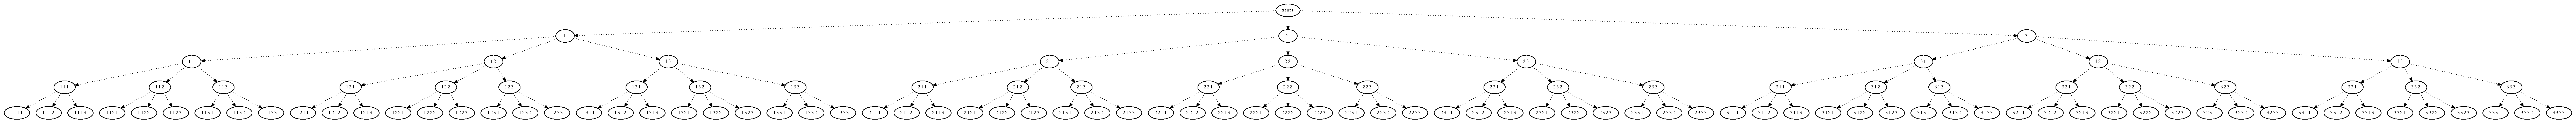
\includegraphics[width=.9\textheight, angle=90]{images/ss1.eps}
\end{center}
\caption{State space tree for the example in table~\ref{t:1}}
\label{fig:ss1}
\end{figure} 

\begin{figure}
\begin{center}
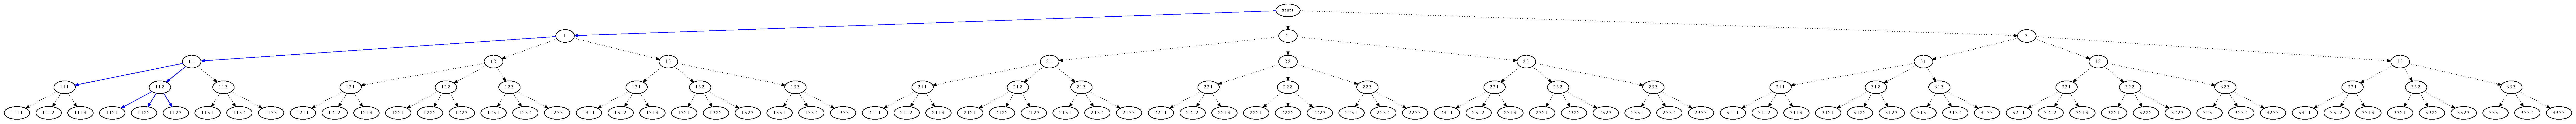
\includegraphics[width=.9\textheight, angle=90]{images/ss2.eps}
\end{center}
\caption{State space tree for the example in table~\ref{t:1}}
\label{fig:ss2}
\end{figure} 


\begin{figure}
\begin{center}
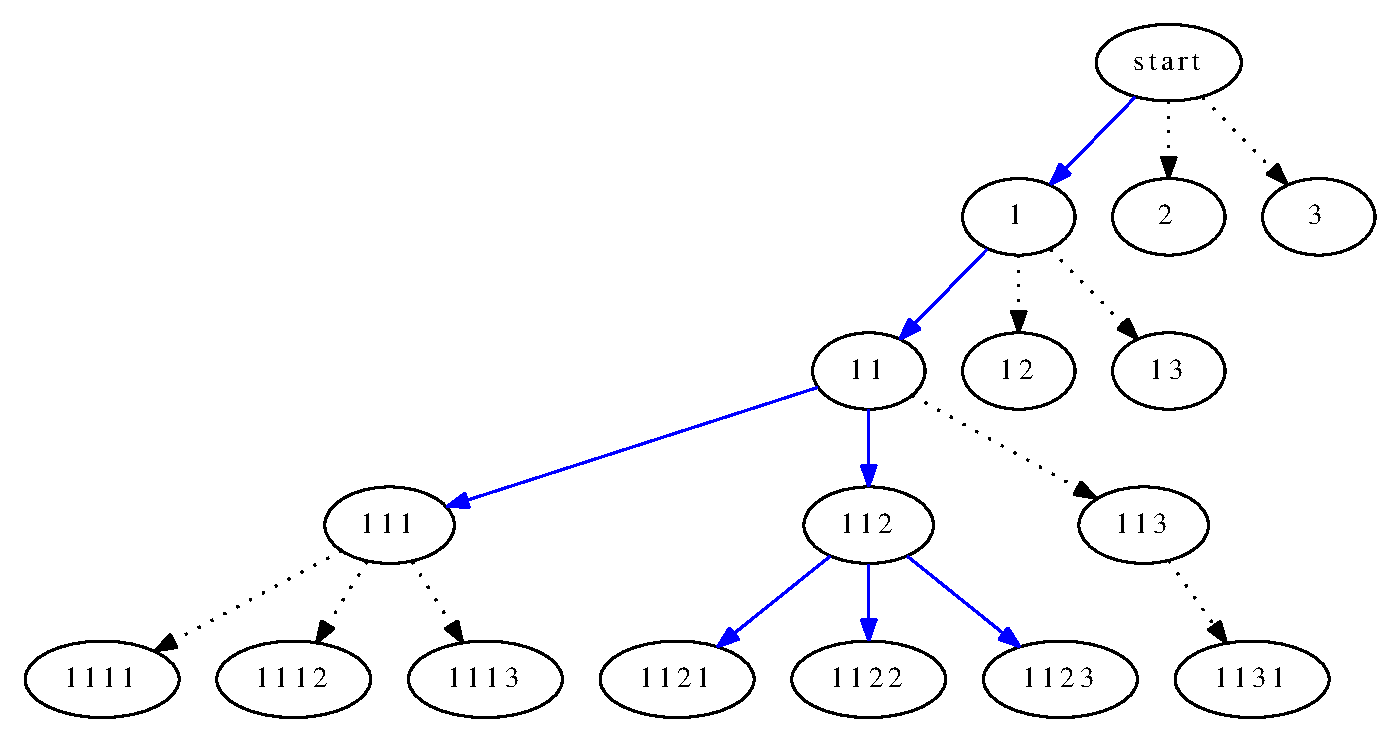
\includegraphics[width=.5\textwidth]{images/ss2-zoom.eps}
\end{center}
\caption{Relevant portion of the state space in figure~\ref{fig:ss2} zoomed in}
\label{fig:ss2-zoom}
\end{figure} 

Figure~\ref{fig:ss1} shows the state space for the scenario considered in table~\ref{t:1}. The state space is represented in the form of a \emph{decision tree}, also called in this context, the \emph{search tree}. Each level in the tree corresponds to a particular course. For example, at level 1, the node labelled 1 means that $c_1$ has been assigned slot $s_1$. At level 2, the node labelled 11 means that $c_1$ has been assigned slot $s_1$ and $c_2$ has been assigned slot $s_1$; at the same level, the node labelled 13 means that $c_1$ has been assigned slot $s_1$ and $c_2$ has been assigned slot $s_3$, and so on. The path from the root to each leaf corresponds to a particular candidate timetable. As explained earlier, the number of candidate timetables in this case is equal to the number of leaves in the search tree, which is $3^4 = 81$.

\subsection{Pruning}
Figure~\ref{fig:ss2} shows the same search tree as in figure~\ref{fig:ss1}, albeit with those edges marked in blue which our algorithm visits during its execution. For convenient reading, the relevant portion of the state space is shown zoomed in in figure~\ref{fig:ss2-zoom}. Note that, on visiting state 111, our algorithm detects a conflict. At this point, it is sure that exploring any part of the sub-tree at 111 would be futile. Therefore, the algorithm leaves out the entire sub-tree of 111 -- a decision which is known as \emph{pruning}. Hence, the algorithm backtracks and visits 112. Then, from there, it proceeds to 1121. Here, on detecting conflict, it backtracks and tries 1122. Here too, a conflict is detected. The algorithm backtracks yet again, finally visiting 1123. Here, no conflict is detected. This being a leaf state corresponds to a solution. This, the algorithm outputs as result. Note that the portion of the state space the algorithm has traversed is a very small portion of the complete state space.

\begin{algorithm}
\caption{Timetable scheduling algorithm}
\label{algo:schedule}
\begin{algorithmic}[1]
\Procedure{satisfy}{$course$, $sched$}
	\State $permitted \gets$ set of non-conflicting slot groups for course in $sched$
	\If{$permitted$ = \textbf{empty}}
		\State \textbf{return empty}
	\EndIf
	\If{$course = $last($courses$)}
		\State $val \gets$ \Call{anyValueIn}{$permitted$}
		\State \textbf{return} $sched \cup $value($course$)=$val$
	\Else
		\For{$val \in permitted$}
			\State $new \gets sched \cup $value($course$)=$val$
			\State $result \gets$ \Call{satisfy}{next($course$), $new$}
			\If{$result \neq$ \textbf{empty}}
				\State \textbf{return} $result$
			\EndIf
		\EndFor
		\State \textbf{return empty}
	\EndIf
	
\EndProcedure

\Statex
\Procedure{schedule}{}
	\State \textbf{return} \Call{satisfy}{first($courses$), \textbf{empty}}
\EndProcedure

\end{algorithmic}
\end{algorithm}

Algorithm~\ref{algo:schedule} presents the pseudo-code of our timetable scheduling algorithm. The $permitted$ set of slots for a course is computed in the context of $sched$ using certain constraints which we call the \emph{hard constraints} and \emph{soft constraints}

Section~\ref{sec:cons} gives more details on what we mean by hard and soft constraints, and how we represent them in our algorithm.

\section{Representing Constraints} \label{sec:cons}
As mentioned above, a $permitted$ set of slots for a course is computed whenever the algorithm. The $satisfy$ is recursively called by augmenting the currently computed schedule (partial) by binding the given course to one value from $permitted$ at a time one by one. The basis of the $permitted$ set are the hard and soft constraints as defined below.
\begin{enumerate}
	\item \textbf{Hard constraints: }For any lecture slot in $permitted$, there is assigned no other course $c$ such that $course$ and $c$ have common participants, i.e. for a schedule $S$, $S \vdash \forall g \in permitted$ and $\forall $ course $c \in g : c \neq course, conflict(course, c) = false$.
	\item \textbf{Soft constraints: }Constraints related the availability and/or convenience of participants are categorised as soft constraints.
\end{enumerate}
 
\subsection{Hard constraints}
\begin{figure}
\begin{center}
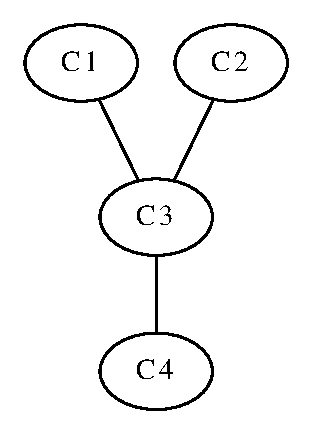
\includegraphics[width=.25\textwidth]{images/cg1.eps}
\end{center}
\caption{Constraint graph for example 1}
\label{fig:cg1}
\end{figure} 

A good way to visualise hard constraints is as \emph{constraint graphs}. An example of a constraint graph corresponding to example 1 is shown in figure~\ref{fig:cg1}. A constraint graph contains a node corresponding to each course. An edge occurs between any two nodes corresponding to courses $c_1$ and $c_2$ if these courses have at least one participant in common. In such a case, nodes corresponding to $c_1$ and $c_2$ are called \emph{neighbours}. To satisfy the hard constraints, we require that no two neighbours  in the constraint graph are scheduled to the same lecture slot.

\subsection{Soft constraints}
In our current implementation, soft constraints are represented as a set of \emph{availability matrices}. One or zero availability matrix may exist for each participant. If, for any participant, the availability matrix is not specified, it means that the participant is available throughout the week for all lecture slots. On the other hand, if an availability matrix exists for a participant, it is to be interpreted as follows: Each row corresponds to a day in a working week. Each column corresponds to a lecture slot. A $1$ means that the corresponding participant is available during that period. Therefore, it is OK to schedule any of the courses that this participant is a part of in that particular slot.

An example of an availability matrix is shown in table~\ref{t:am}. For instance, there's a $0$ in the cell [\textbf{Thu}, \textbf{L3}] meaning that the given participant is unavailable in the lecture slot L3 on Thursdays. On the other hand, there's a $1$ in the cell [\textbf{Fri}, \textbf{L2}] meaning that the given participant is available in the lecture slot L2 on Fridays.
  
\begin{table}
\begin{center}

\begin{tabular}{l | c | c | c | c}
    & \textbf{L1} & \textbf{L2} & \textbf{L3} & \textbf{L4} \\
\hline
\textbf{Mon} & 1  & 1  & 1  & 0 \\
\textbf{Tue} & 1  & 1  & 1  & 0 \\
\textbf{Wed} & 1  & 1  & 0  & 0 \\
\textbf{Thu} & 1  & 1  & 0  & 0 \\
\textbf{Fri} & 1  & 1  & 0  & 0 \\
\textbf{Sat} & 0  & 0  & 0  & 0

\end{tabular}
\end{center}
\caption{Availability Matrix: an example}
\label{t:am}
\end{table}

\subsection{Advantages and Limitations}
We mentioned earlier that the timetable scheduling problem is NP-complete. Therefore all attempts to design an efficient algorithm giving the best result would most likely fail. In view of this, following is a list of some advantages of our algorithm:

\begin{enumerate}
	\item The \textsf{schedule} algorithm performs an exhaustive search. Therefore, it is sure to find a solution if it exists. In the worst case, this may take unacceptably long, but in general, this doesn't happen.
	\item Due to typical characteristics of a practical problem instance, our algorithm is able to come back with a solution fairly quickly.
	\item Soft constraints can be plugged into and out of the algorithm as needed fairly conveniently.
	\item The branch and bound structure of our algorithm is amenable to parallelisation. The problem can be naturally divided along the branches of the search tree, each of which could then be independently solved by parallelly running threads.
\end{enumerate}



However, there are some limitations:
\begin{enumerate}
	\item The worse case performance of \textsf{schedule} is exponential.
	\item If, under the given soft constraints, the algorithm fails to compute a solution, there is no hint regarding which constraint plays a role in causing the failure.
	\item The algorithm has a randomised element to it. Consequently, it may result in different solutions every time it is run on the same problem instance.
	\item The randomised element also makes it difficult to track the progress of the computation. This becomes a problem when we want to throw away a solution it provides and wish to continue searching that point on. It is possible to preserve the state of computation by preserving the already traversed part of the search tree. But this will result in an explosion in the memory requirement of the program. There may be ways of optimising the storage of the search tree, but we are currently unaware of any such method.
\end{enumerate}

\section{Experimental Results}
%\begin{quotation}
%\emph{The career of this young and talented algorithm came to a premature end when he met with a tragic end in a massive explosion: {\color{red} THE STATE SPACE EXPLOSION!}}
%\end{quotation}


We implemented our timetable scheduling algorithm in a prototype application written in python. We ran it over a real course registration data set from one of the recent semesters in our institute. There were 64 courses offered in that semester. Each had to be assigned 2 lectures per week. The entire work-week spanned six days (Monday through to Friday) with four lecture slots daily, resulting in 24 lecture slots in a week. The state space is, therefore, fairly massive in size: $24^{64}$ states. There were additional soft constraints, but in our initial run, we didn't include them. As it turned out, the algorithm didn't return with a result even after running non-stop for 2 days after which we killed it. We concluded that that the algorithm is not able to handle complexity of practical scale.
\section{Related Work}

\section{Conclusion}
We have presented a branch and bound algorithm for the timetable scheduling problem. We have demonstrated that, even though the problem is inherently intractable, our algorithm is able to fair well in scenarios of practical scale. The reason for this is that the search tree pruning allows us to omit large parts of the state space from our search. Also, as the constraints become larger in number, the search tree shrinks in its width deflating the state space further. In a reasonable scenario, the constraint graph is sparse enough that we are able to hit our solution fairly early in our search process most of the times. Where the problem instance is very tightly constrained, where the solutions are far and between, this approach would perform much better in searching them out than a human scheduler.


\end{document}